% !TEX program = xelatex
\documentclass[UTF8,fontset=fandol,a4paper,11pt]{ctexart}
\usepackage[margin=21mm,top=23mm,bottom=22mm,headheight=16pt]{geometry}
\usepackage{amsmath,amssymb,mathtools,bm}
\usepackage{tikz}
\usetikzlibrary{arrows.meta,calc,angles,quotes,patterns}
\usepackage{xcolor,booktabs,array,longtable,enumitem,fancyhdr,needspace}
\usepackage[unicode,hidelinks]{hyperref}
\definecolor{ink}{HTML}{24343C}
\definecolor{accent}{HTML}{166A70}
\definecolor{muted}{HTML}{65747A}
\definecolor{rulegray}{HTML}{D4DDE0}
\definecolor{warm}{HTML}{966037}
\color{ink}
\setlength{\parindent}{2em}
\setlength{\parskip}{4pt}
\linespread{1.12}
\AtBeginDocument{\setlength{\abovedisplayskip}{6pt plus 2pt minus 1pt}
\setlength{\belowdisplayskip}{6pt plus 2pt minus 1pt}
\setlength{\abovedisplayshortskip}{0pt plus 1pt}
\setlength{\belowdisplayshortskip}{4pt plus 1pt}}
\setlist[enumerate]{label=(\arabic*),leftmargin=2.3em,itemsep=3pt,topsep=4pt}
\setlist[itemize]{leftmargin=2em,itemsep=2pt,topsep=4pt}
\allowdisplaybreaks[1]
\setlength{\emergencystretch}{2em}
\setcounter{secnumdepth}{0}
\providecommand{\tightlist}{\setlength{\itemsep}{0pt}\setlength{\parskip}{0pt}}
\ctexset{section={format=\Large\bfseries\color{accent},beforeskip=10pt,afterskip=9pt},
subsection={format=\normalsize\bfseries\color{accent},beforeskip=10pt,afterskip=4pt},
subsubsection={format=\normalsize\bfseries,beforeskip=8pt,afterskip=3pt}}
\pagestyle{fancy}
\fancyhf{}
\fancyhead[L]{\small\color{muted}物理学难题集萃}
% 页眉仅保留书名；版本名称只在封面显示。
\fancyfoot[L]{\small\color{muted}\chapterlabel}
\fancyfoot[R]{\small\thepage}
\renewcommand{\headrulewidth}{0.4pt}
\renewcommand{\footrulewidth}{0pt}
\newcommand{\dd}{\mathop{}\!\mathrm{d}}
\newcommand{\vect}[1]{\bm{#1}}
\newcommand{\tagline}[1]{\noindent{\small\color{muted}#1}\par}
\newcommand{\result}[1]{\begin{equation*}\boxed{#1}\end{equation*}}
\newcommand{\figcaption}[1]{\par\vspace{2pt}{\small\color{muted}#1}\par}
\newcommand{\teach}[2]{\Needspace{4\baselineskip}\subsection*{讲解要点与追问}#1\par\smallskip\noindent\textbf{追问：}#2\par}
\newcommand{\workarea}{\par\vspace{7mm}\noindent{\small\color{muted}作答区}\par\vspace{4mm}
\noindent\textcolor{rulegray}{\rule{\linewidth}{0.3pt}}\par\vspace{16mm}
\noindent\textcolor{rulegray}{\rule{\linewidth}{0.3pt}}\par\vspace{16mm}
\noindent\textcolor{rulegray}{\rule{\linewidth}{0.3pt}}\par\vspace{16mm}
\noindent\textcolor{rulegray}{\rule{\linewidth}{0.3pt}}}
\tikzset{axis/.style={-{Stealth[length=2mm]},thin,color=muted},
motion/.style={-{Stealth[length=2.3mm]},thick,color=accent},
force/.style={-{Stealth[length=2.3mm]},thick,color=warm},
traj/.style={thick,color=accent},guide/.style={dashed,thin,color=muted},
object/.style={thick,color=ink},every node/.style={font=\small}}\widowpenalty=10000\clubpenalty=10000\displaywidowpenalty=10000\newcommand{\chapterlabel}{电磁学试题（四）}







\hypersetup{pdftitle={电磁学试题（四）·学生版},pdfauthor={}}

\begin{document}\pdfbookmark[0]{电磁学试题（四）}{cover}

\thispagestyle{empty}\vspace*{22mm}

\noindent{\Huge\bfseries 物理学难题集萃}\par\vspace{12mm}

\noindent{\LARGE 电磁学试题（四）}\par\vspace{12mm}

\noindent{\Large\color{accent}学生版}\par\vspace{9mm}

\noindent\textcolor{accent}{\rule{\linewidth}{1pt}}\par\vspace{9mm}

\noindent 第1--5题\par\vfill\clearpage

\pdfbookmark[1]{题目目录}{contents}\section*{题目目录}

\begin{longtable}{@{}r p{113mm} r@{}}\toprule 题号 & 题目 & 页码\\\midrule

\hyperref[q:1]{1} & \hyperref[q:1]{非均匀导体中的体电荷与界面电荷} & \pageref{q:1} \\

\hyperref[q:2]{2} & \hyperref[q:2]{多端等效与无限内接三角形网络} & \pageref{q:2} \\

\hyperref[q:3]{3} & \hyperref[q:3]{互补RL、RC支路的相量与初始储能} & \pageref{q:3} \\

\hyperref[q:4]{4} & \hyperref[q:4]{双行CLC网络的复阻抗和功率因数} & \pageref{q:4} \\

\hyperref[q:5]{5} & \hyperref[q:5]{导体屏蔽暂态与单频等效电容} & \pageref{q:5} \\

\bottomrule\end{longtable}

\clearpage

\pdfbookmark[2]{第 1 题 非均匀导体中的体电荷与界面电荷}{q1}

\section*{第 1 题\quad 非均匀导体中的体电荷与界面电荷}\label{q:1}


长为$L$、截面积为$S$的均匀粗细导体，沿轴线$x$的电阻率为
\[
\rho(x)=\rho_0\left|\sin\frac{2\pi x}{L}\right|,\qquad 0\le x\le L.
\]
导体两端保持电势差$V(0)-V(L)=U>0$，已达稳恒状态。采用一维导电模型，电场沿轴线，电荷关系用$\varepsilon_0$描述。
\begin{enumerate}
\item 求导体电阻和电流密度。
\item 求内部体电荷密度$\rho_e(x)$，指出带正电的区段。
\item $x=L/2$处体电荷密度发生跳变，该截面上是否存在面电荷？给出判断依据。
\end{enumerate}


\begin{center}\begin{minipage}{.98\linewidth}\centering
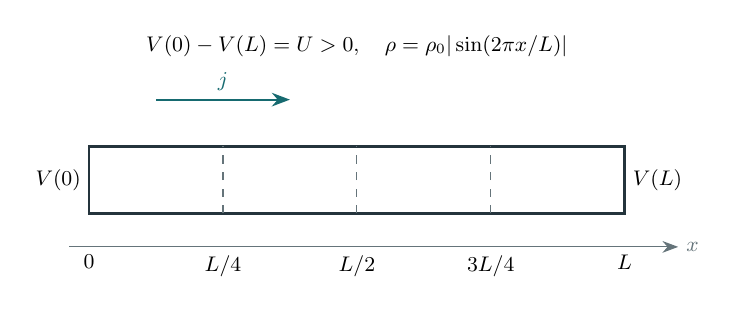
\begin{tikzpicture}[scale=.85,transform shape]

\draw[object] (0,-.5) rectangle (8,.5);
\foreach \x in {2,4,6}{\draw[guide] (\x,-.5)--(\x,.5);}
\draw[motion] (1,1.2)--(3,1.2) node[midway,above] {$j$};
\draw[axis] (-.3,-1)--(8.8,-1) node[right] {$x$};
\foreach \x/\l in {0/0,2/{L/4},4/{L/2},6/{3L/4},8/L}{\node[below] at (\x,-1) {$\l$};}
\node[left] at (0,0) {$V(0)$};\node[right] at (8,0) {$V(L)$};
\node at (4,2) {$V(0)-V(L)=U>0,\quad \rho=\rho_0|\sin(2\pi x/L)|$};

\end{tikzpicture}
\figcaption{图电试4.1\quad 同截面微段串联，稳恒电流沿轴向。}
\end{minipage}\end{center}

\par\vspace{5mm}\noindent{\small\color{muted}作答区}\par\vspace{3mm}\noindent\textcolor{rulegray}{\rule{\linewidth}{0.3pt}}\par\vspace{12mm}\noindent\textcolor{rulegray}{\rule{\linewidth}{0.3pt}}

\clearpage

\pdfbookmark[2]{第 2 题 多端等效与无限内接三角形网络}{q2}

\section*{第 2 题\quad 多端等效与无限内接三角形网络}\label{q:2}


\begin{enumerate}
\item $N$端电阻网络可用外端两两之间的等效支路表示。说明这种表示中何时须允许开路支路，画出四端完全网络，以及一个由八个电阻组成、不能直接串并联约化的四端网络。
\item 等边三角形$ABC$的三边均被中点$P,Q,T$分为两段，每段电阻为$R$，三个中点之间也各接一个电阻$R$，其中$P$在$AB$、$Q$在$BC$、$T$在$CA$。求其对外端$A,B,C$的对称三角形等效网络。
\item 两个边长$a$的等边三角形$ABC$与$BCD$共边$BC$。左三角形中不断连接三边中点构成内接三角形，所有中点均电连接；右侧只增加$CD,DB$两段。各段为相同材料和粗细的金属丝，单位长度电阻$r$。求全网络$A,B$间等效电阻。
\end{enumerate}
无限网络按有限层截断、最内层不再加支路的极限定义。


\begin{center}\begin{minipage}{.98\linewidth}\centering
\begin{tikzpicture}[scale=.7,transform shape]

\coordinate (A) at (0,0);\coordinate (B) at (4,0);\coordinate (C) at (2,3.464);
\coordinate (P) at (2,0);\coordinate (Q) at (3,1.732);\coordinate (T) at (1,1.732);
\draw[object] (A)--(B)--(C)--cycle;\draw[object] (P)--(Q)--(T)--cycle;
\foreach \p/\pos in {A/below left,B/below right,C/above,P/below,Q/right,T/left}{\fill (\p) circle (1.6pt) node[\pos] {$\p$};}
\node at (2,-1) {每一小段均为$R$};\begin{scope}[xshift=7cm]
\coordinate (A) at (0,0);\coordinate (B) at (4,0);\coordinate (C) at (2,3.464);
\coordinate (D) at (6,3.464);
\draw[object] (A)--(B)--(C)--cycle;\draw[object] (C)--(D)--(B);
\foreach \k in {1,...,7}{
\coordinate (M) at ($(A)!.5!(B)$);\coordinate (N) at ($(B)!.5!(C)$);\coordinate (O) at ($(C)!.5!(A)$);
\draw[object] (M)--(N)--(O)--cycle;
\coordinate (A) at (M);\coordinate (B) at (N);\coordinate (C) at (O);}
\node[below left] at (0,0) {$A$};\node[below] at (4,0) {$B$};
\node[above] at (2,3.464) {$C$};\node[above right] at (6,3.464) {$D$};
\node[above] at (4,3.464) {$k=ar$};\node[right] at (5,1.732) {$k$};
\node at (3,-1) {左部无限内接，右部仅加两边};\end{scope}
\end{tikzpicture}
\figcaption{图电试4.2\quad 有限九电阻三角形与共边的无限三角形组合。}
\end{minipage}\end{center}

\par\vspace{5mm}\noindent{\small\color{muted}作答区}\par\vspace{3mm}\noindent\textcolor{rulegray}{\rule{\linewidth}{0.3pt}}\par\vspace{12mm}\noindent\textcolor{rulegray}{\rule{\linewidth}{0.3pt}}

\clearpage

\pdfbookmark[2]{第 3 题 互补RL、RC支路的相量与初始储能}{q3}

\section*{第 3 题\quad 互补RL、RC支路的相量与初始储能}\label{q:3}


一电源给两条并联支路供电：一条为电阻$R$与电感$L$串联，另一条为电阻$R$与电容$C$串联。元件理想，电源内阻忽略。
\begin{enumerate}
\item 电动势$\mathcal E(t)=\mathcal E_0\sin^2\omega t$，且$\omega L=1/(\omega C)=R$。用相量图分析稳态两支路电流及总电流。
\item 电动势为具有傅里叶展开的任意周期函数。$L,C,R$满足什么关系时，稳态端口电流总为$i(t)=\mathcal E(t)/R$？用复导纳证明。
\item 在第（2）问所求匹配关系下，给出任意初始电感电流$i_L(0)$与电容电压$v_C(0)$时的端口电流，说明稳态结论的初始条件限制。
\end{enumerate}
电容电压取沿支路电流方向的电势降。


\begin{center}\begin{minipage}{.98\linewidth}\centering
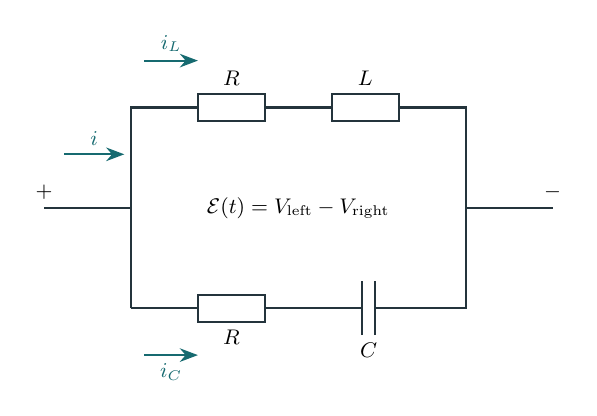
\begin{tikzpicture}[scale=.85,transform shape]

\draw[object] (0,0)--(0,3)--(1,3);
\draw[object] (1,2.8) rectangle (2,3.2);\node[above] at (1.5,3.2) {$R$};
\draw[object] (2,3)--(3,3);\draw[object] (3,2.8) rectangle (4,3.2);\node[above] at (3.5,3.2) {$L$};
\draw[object] (4,3)--(5,3)--(5,0)--(4,0);
\draw[object] (3.45,-.4)--(3.45,.4);\draw[object] (3.65,-.4)--(3.65,.4);
\draw[object] (4,0)--(3.65,0);\draw[object] (3.45,0)--(2,0);
\draw[object] (1,-.2) rectangle (2,.2);\node[below] at (1.5,-.2) {$R$};
\draw[object] (1,0)--(0,0);
\draw[object] (0,1.5)--(-1.3,1.5);\draw[object] (5,1.5)--(6.3,1.5);
\draw[motion] (-1,2.3)--(-.1,2.3) node[midway,above] {$i$};
\draw[motion] (.2,3.7)--(1,3.7) node[midway,above] {$i_L$};
\draw[motion] (.2,-.7)--(1,-.7) node[midway,below] {$i_C$};
\node[below] at (3.55,-.4) {$C$};
\node[above] at (-1.3,1.5) {$+$};\node[above] at (6.3,1.5) {$-$};
\node at (2.5,1.5) {$\mathcal E(t)=V_{\rm left}-V_{\rm right}$};

\end{tikzpicture}
\figcaption{图电试4.3\quad 两串联支路共用端电压，电流正方向均从左到右。}
\end{minipage}\end{center}

\par\vspace{5mm}\noindent{\small\color{muted}作答区}\par\vspace{3mm}\noindent\textcolor{rulegray}{\rule{\linewidth}{0.3pt}}\par\vspace{12mm}\noindent\textcolor{rulegray}{\rule{\linewidth}{0.3pt}}

\clearpage

\pdfbookmark[2]{第 4 题 双行CLC网络的复阻抗和功率因数}{q4}

\section*{第 4 题\quad 双行CLC网络的复阻抗和功率因数}\label{q:4}


如图，两条水平支路各依次由电容$C$、电感$L$、电容$C$连接而成；四列上下对应结点之间均接电阻$R$。以左下结点$A$和右上结点$B$为端口。
\begin{enumerate}
\item 求角频率$\omega$下的端口复阻抗$Z$。
\item 当$\omega L=1/(\omega C)=R$时，求$|Z|$和功率因数，说明电流相位。
\end{enumerate}
所有同名元件参数相同；用电流从$A$流入、从$B$流出的方向定义端口电压。


\begin{center}\begin{minipage}{.98\linewidth}\centering
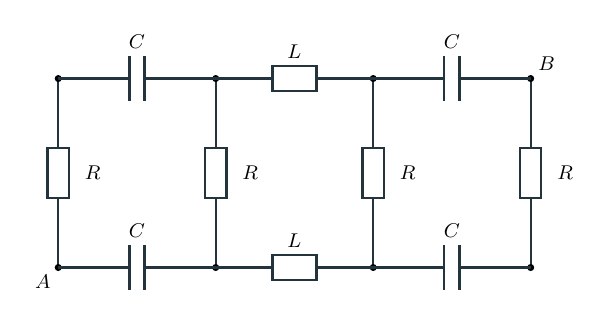
\begin{tikzpicture}[scale=.8,transform shape]

\foreach \x in {0,2.5,5,7.5}{
\draw[object] (\x,0)--(\x,1.1);
\draw[object] ({\x-.17},1.1) rectangle ({\x+.17},1.9);
\draw[object] (\x,1.9)--(\x,3);
\node[right] at ({\x+.3},1.5) {$R$};
\fill (\x,0) circle (1.6pt);\fill (\x,3) circle (1.6pt);}
\foreach \y in {0,3}{
\foreach \a/\b in {0/2.5,5/7.5}{
\pgfmathsetmacro{\m}{(\a+\b)/2}
\draw[object] (\a,\y)--({\m-.12},\y);
\draw[object] ({\m+.12},\y)--(\b,\y);
\draw[object] ({\m-.12},{\y-.35})--({\m-.12},{\y+.35});
\draw[object] ({\m+.12},{\y-.35})--({\m+.12},{\y+.35});
\node[above] at (\m,{\y+.35}) {$C$};}
\draw[object] (2.5,\y)--(3.4,\y);
\draw[object] (3.4,{\y-.2}) rectangle (4.1,{\y+.2});
\draw[object] (4.1,\y)--(5,\y);\node[above] at (3.75,{\y+.2}) {$L$};}
\node[below left] at (0,0) {$A$};\node[above right] at (7.5,3) {$B$};

\end{tikzpicture}
\figcaption{图电试4.4\quad 上下均为CLC，四列竖直电阻相同；端口在对角两端。}
\end{minipage}\end{center}

\par\vspace{5mm}\noindent{\small\color{muted}作答区}\par\vspace{3mm}\noindent\textcolor{rulegray}{\rule{\linewidth}{0.3pt}}\par\vspace{12mm}\noindent\textcolor{rulegray}{\rule{\linewidth}{0.3pt}}

\clearpage

\pdfbookmark[2]{第 5 题 导体屏蔽暂态与单频等效电容}{q5}

\section*{第 5 题\quad 导体屏蔽暂态与单频等效电容}\label{q:5}


长$l$、截面积$S$的导体，在一维平行面近似下置于沿轴线的外加电场中。$t<0$时无电场且无表面电荷；$t=0$起外加电场为
$E_{\rm ext}(t)=E_0\cos\omega t$。导体电导率为$\sigma=\alpha\varepsilon_0\omega$，$\alpha>0$；在本题给定频率，$\sigma$为实常量。忽略边缘效应、传播延迟及载流子惯性。
\begin{enumerate}
\item 求导体中的传导电流密度$j(t)$，并给出表面电荷随时间的变化。
\item 暂态消失后，以外加电势降$u_{\rm ext}(t)=lE_{\rm ext}(t)$为输入、传导电流$i(t)=Sj(t)$为输出，求单频并联电阻$R_p$与电容$C_p$的等效值。
\item 在普通准静态、无色散且相对介电常数$\varepsilon_r\ge1$的介质模型内，能否用相同$l,S$的一个填充介质电容实现该$C_p$？说明该比较的适用范围，并给出可实现端口等效的电阻、电容网络。
\end{enumerate}
导体内部总电场包含表面电荷的屏蔽场；这里输出专指传导电流。


\begin{center}\begin{minipage}{.98\linewidth}\centering
\begin{tikzpicture}[scale=.9,transform shape]

\fill[muted!8] (0,-1) rectangle (6,1);
\draw[object] (0,-1) rectangle (6,1);
\draw[object] (0,-1.2)--(0,1.2);\draw[object] (6,-1.2)--(6,1.2);
\foreach \y in {-.65,0,.65}{\node[left] at (0,\y) {$-$};\node[right] at (6,\y) {$+$};}
\node[above] at (0,1.2) {$-s$};\node[above] at (6,1.2) {$s$};
\draw[motion] (1,2.2)--(5,2.2) node[midway,above] {$E_{\rm ext}=E_0\cos\omega t$};
\draw[force] (4,.1)--(2,.1) node[midway,above] {$E_{\rm ind}=-s/\varepsilon_0$};
\draw[axis,<->] (0,-1.8)--(6,-1.8) node[midway,below] {$l$};
\node at (3,-3) {一维平行面近似；截面积$S$};

\end{tikzpicture}
\figcaption{图电试4.5\quad 场箭头按外场与右端正电荷均为正时示意，实际符号随时间变化。}
\end{minipage}\end{center}

\par\vspace{5mm}\noindent{\small\color{muted}作答区}\par\vspace{3mm}\noindent\textcolor{rulegray}{\rule{\linewidth}{0.3pt}}\par\vspace{12mm}\noindent\textcolor{rulegray}{\rule{\linewidth}{0.3pt}}

\end{document}
